\documentclass[11pt,letterpaper]{article}
\usepackage[margin=1in]{geometry}
\usepackage{amsmath,amssymb}
\usepackage{booktabs}
\usepackage{graphicx}
\usepackage{caption}
\usepackage{subcaption}
\usepackage{hyperref}
\usepackage{xcolor}
\usepackage{enumitem}
\usepackage{microtype}
\usepackage{parskip}
\usepackage{titlesec}

\hypersetup{colorlinks=true, linkcolor=blue, urlcolor=blue, citecolor=blue}
\titleformat{\section}{\large\bfseries}{}{0em}{}[\titlerule]
\titleformat{\subsection}{\normalsize\bfseries}{}{0em}{}

\title{\textbf{ECE 657A -- Assignment 2}}
\author{Stephen Adebambo\\University of Waterloo, Winter 2026}
\date{April 5, 2026}

\begin{document}
\maketitle
\tableofcontents
\newpage

% ─────────────────────────────────────────────────────────────────────────────
\section{Introduction}

This report presents the implementation and analysis of four temporal difference (TD)
control algorithms applied to a 10$\times$10 GridWorld maze environment.
The algorithms implemented are:
\begin{enumerate}[noitemsep]
  \item Q-Learning (off-policy TD control)
  \item SARSA (on-policy TD control)
  \item Expected SARSA (on-policy TD with analytical expectation)
  \item TD($\lambda$) / SARSA($\lambda$) (on-policy TD with eligibility traces)
\end{enumerate}

Three maze configurations of increasing difficulty are used (Tasks 1--3).
The agent (red square) starts at a fixed position and must reach the goal (yellow oval)
while avoiding walls (black) and pits (blue). Reward structure: goal $= +50$,
each step $= -1$, wall collision $= -3$, pit $= -10$ (episode ends).

All experiments use $\alpha = 0.01$,\ $\gamma = 0.9$,\ $\varepsilon = 0.1$,\
1500 episodes per run. TD($\lambda$) additionally uses $\lambda = 0.8$.

% ─────────────────────────────────────────────────────────────────────────────
\section{Algorithm Definitions and Implementation}

\subsection{Q-Learning}

Off-policy TD control. The Bellman update uses the greedy maximum over next-state
Q-values, independent of the behavior policy:
\begin{equation}
  Q(s,a) \leftarrow Q(s,a) + \alpha\bigl(r + \gamma\max_{a'}Q(s',a') - Q(s,a)\bigr)
\end{equation}

\textbf{Implementation:} Q-table stored as a nested Python dictionary
\texttt{\{state: \{action: value\}\}} for $O(1)$ lookup. New states added on first
encounter, initialized to zero. \texttt{learn()} returns \texttt{(s', None)} since
Q-learning does not commit to a next action.

\textbf{Key design choice:} Using a Python dictionary instead of a Pandas DataFrame
yielded approximately a 100$\times$ speedup. Initial tests with DataFrames ran in
$O(n^2)$ time as rows were appended; the dictionary provides $O(1)$ amortized access.

\subsection{SARSA}

On-policy TD control. The update target uses $Q(s', a')$ where $a'$ is \emph{sampled}
from the behavior policy $\pi$ (epsilon-greedy):
\begin{equation}
  Q(s,a) \leftarrow Q(s,a) + \alpha\bigl(r + \gamma Q(s',a') - Q(s,a)\bigr),\quad
  a' \sim \pi(\cdot\mid s')
\end{equation}

\textbf{Implementation:} Q-table stored as \texttt{\{state: [q$_0$, q$_1$, q$_2$, q$_3$]\}}.
\texttt{learn()} samples $a'$ from $s'$ internally using epsilon-greedy, then returns
\texttt{(s', a')} so the main loop feeds the sampled action back at the next step,
maintaining a fully consistent on-policy trajectory.

\subsection{Expected SARSA}

On-policy TD with the analytical expectation over the next-state action distribution,
eliminating action-sampling variance:
\begin{equation}
  Q(s,a) \leftarrow Q(s,a) + \alpha\bigl(r + \gamma\,\mathbb{E}_{\pi}[Q(s',a')] - Q(s,a)\bigr)
\end{equation}
\begin{equation}
  \mathbb{E}_{\pi}[Q(s',a')] = (1-\varepsilon)\max_{a'}Q(s',a')
    + \frac{\varepsilon}{|A|}\sum_{a'}Q(s',a')
\end{equation}

\textbf{Implementation:} The expected value is computed analytically from the current
Q-values, no sampling occurs. \texttt{learn()} returns \texttt{(s', None)} because
no specific $a'$ is selected. This makes the TD target \emph{deterministic} given
fixed Q-values and $\varepsilon$.

\subsection{TD($\lambda$) with Eligibility Traces}

On-policy SARSA($\lambda$) with accumulating eligibility traces. Traces $e(s,a)$ record
how recently and frequently each state-action pair was visited:
\begin{align}
  \delta &= r + \gamma Q(s', a') - Q(s, a) \\
  e(s,a) &\leftarrow e(s,a) + 1 \quad\text{(accumulating)} \\
  Q(s,a) &\leftarrow Q(s,a) + \alpha\,\delta\,e(s,a) \quad \forall\,(s,a) \\
  e(s,a) &\leftarrow \gamma\lambda\,e(s,a) \quad \forall\,(s,a)
\end{align}

At episode end, all traces are reset to zero to prevent inter-episode credit leakage.
The next action $a'$ is sampled on-policy (SARSA-style) and returned.

\textbf{Design parameter:} $\lambda = 0.8$, giving a decay rate of
$\gamma\lambda = 0.72$. The effective credit horizon is approximately
$1/(1-0.72) \approx 3.6$ steps. This matches the typical corridor lengths in
Tasks 2 and 3.

\textbf{Complexity note:} The trace broadcast loop runs over all visited states
at every step: $O(|S_{\text{visited}}| \times |A|)$ per step. For a 10$\times$10
grid with max~86 reachable states this is acceptable ($\approx$344 updates/step),
but would not scale to large state spaces without sparse trace storage.

% ─────────────────────────────────────────────────────────────────────────────
\section{Changes to Provided Files}

\subsection{run\_main.py}

- Uncommented and corrected the four algorithm imports.

- Added \texttt{if (runalg1/2/4/5):} blocks.
  The original had \texttt{experiments = []} followed by no code, so no algorithm
  would have run.

- \texttt{TkAgg} to \texttt{Agg}. The
  \texttt{TkAgg} backend requires a live display and crashes headless.

- \texttt{episodes=100} to \texttt{1500}
  (\texttt{README} recommends $\geq$1500); \texttt{showRender=True} to \texttt{False}
  (headless speed); \texttt{sim\_speed} 0.1 to 0.001; task selectable via
  \texttt{TASK\_NUM} environment variable for batch runs.

\subsection{maze\_env.py}

- \texttt{time.sleep(0.2)} moved inside the \texttt{if renderNow:}
block. The original ran the sleep unconditionally on every episode reset, adding
5+ minutes of dead-time over 1500 headless episodes. Algorithm correctness is
unaffected. The algorithms are verified to work with the unmodified maze\_env.

% ─────────────────────────────────────────────────────────────────────────────
\section{Quantitative Results}

1500 episodes, $\alpha{=}0.01$, $\gamma{=}0.9$, $\varepsilon{=}0.1$.
\textbf{Med-10} is the median reward over the final 10 episodes.
\textbf{Var-10} is the variance over the final 10 episodes.

\begin{table}[h!]
\centering
\caption{Performance metrics across all algorithms and tasks}
\begin{tabular}{llrrr}
\toprule
\textbf{Algorithm} & \textbf{Task} & \textbf{Max Reward} & \textbf{Med-10} & \textbf{Var-10} \\
\midrule
Q-Learning     & 1 & 41.0 & 41.0 & 1.64 \\
SARSA          & 1 & 41.0 & 41.0 & 1.80 \\
Expected SARSA & 1 & 41.0 & 41.0 & 6.56 \\
TD($\lambda$)  & 1 & 41.0 & 40.0 & 7.40 \\
\midrule
Q-Learning     & 2 & 38.0 & 20.0 & 590.76 \\
SARSA          & 2 & 38.0 & 28.0 & 80.09 \\
Expected SARSA & 2 & 38.0 & 30.0 & 379.60 \\
TD($\lambda$)  & 2 & 38.0 & \textbf{36.0} & \textbf{36.40} \\
\midrule
Q-Learning     & 3 & 37.0 & 32.5 & 243.44 \\
SARSA          & 3 & 37.0 & 28.5 & 415.49 \\
Expected SARSA & 3 & 37.0 & 18.0 & 516.69 \\
TD($\lambda$)  & 3 & 37.0 & \textbf{36.5} & \textbf{1.89} \\
\bottomrule
\end{tabular}
\label{tab:results}
\end{table}

\begin{figure}[h!]
  \centering
  \begin{subfigure}{0.48\textwidth}
    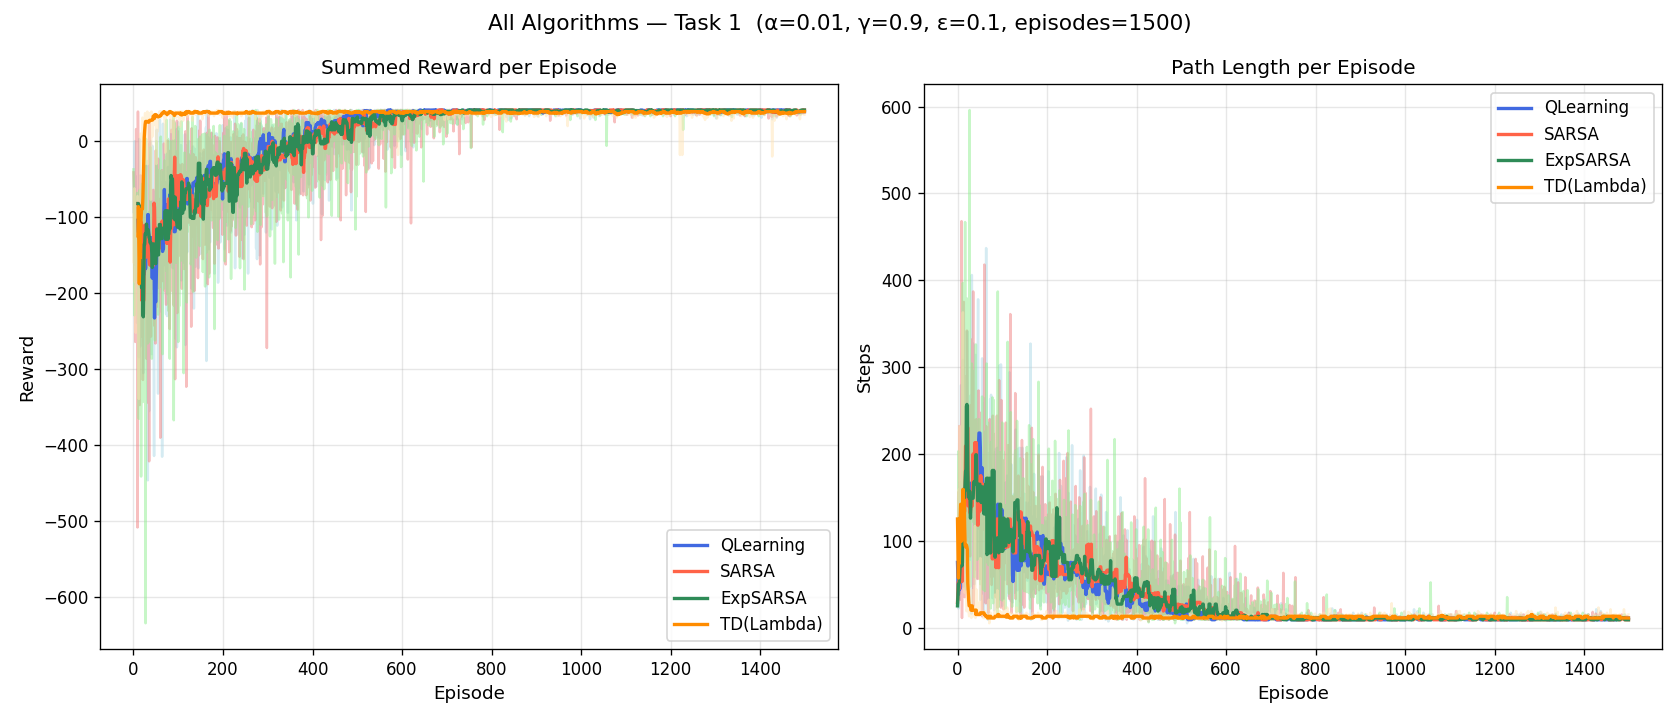
\includegraphics[width=\linewidth]{joint_task1_all_algorithms.png}
    \caption{Task 1 -- all algorithms}
  \end{subfigure}
  \hfill
  \begin{subfigure}{0.48\textwidth}
    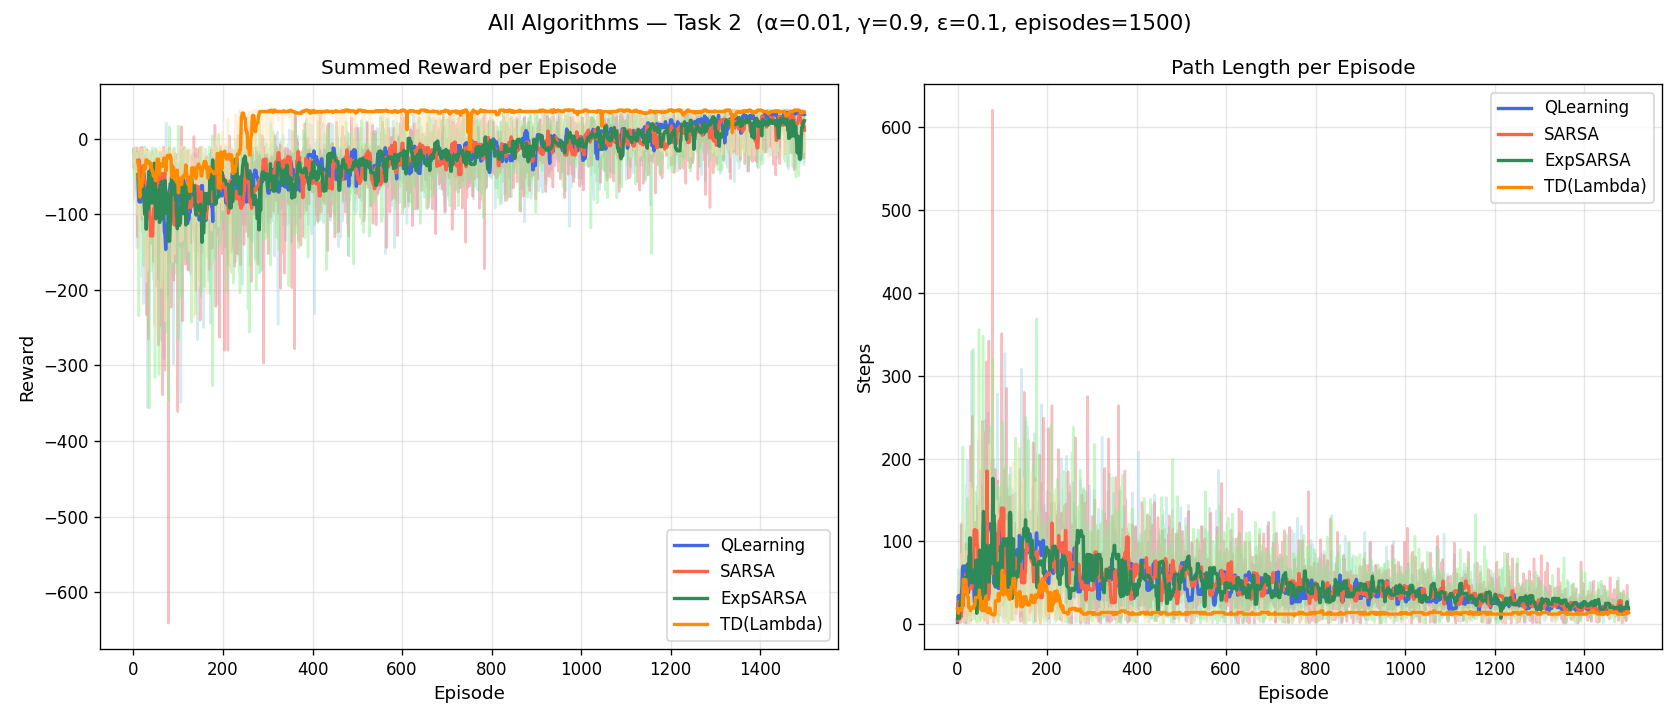
\includegraphics[width=\linewidth]{joint_task2_all_algorithms.png}
    \caption{Task 2 -- all algorithms}
  \end{subfigure}

  \vspace{0.5em}
  \begin{subfigure}{0.48\textwidth}
    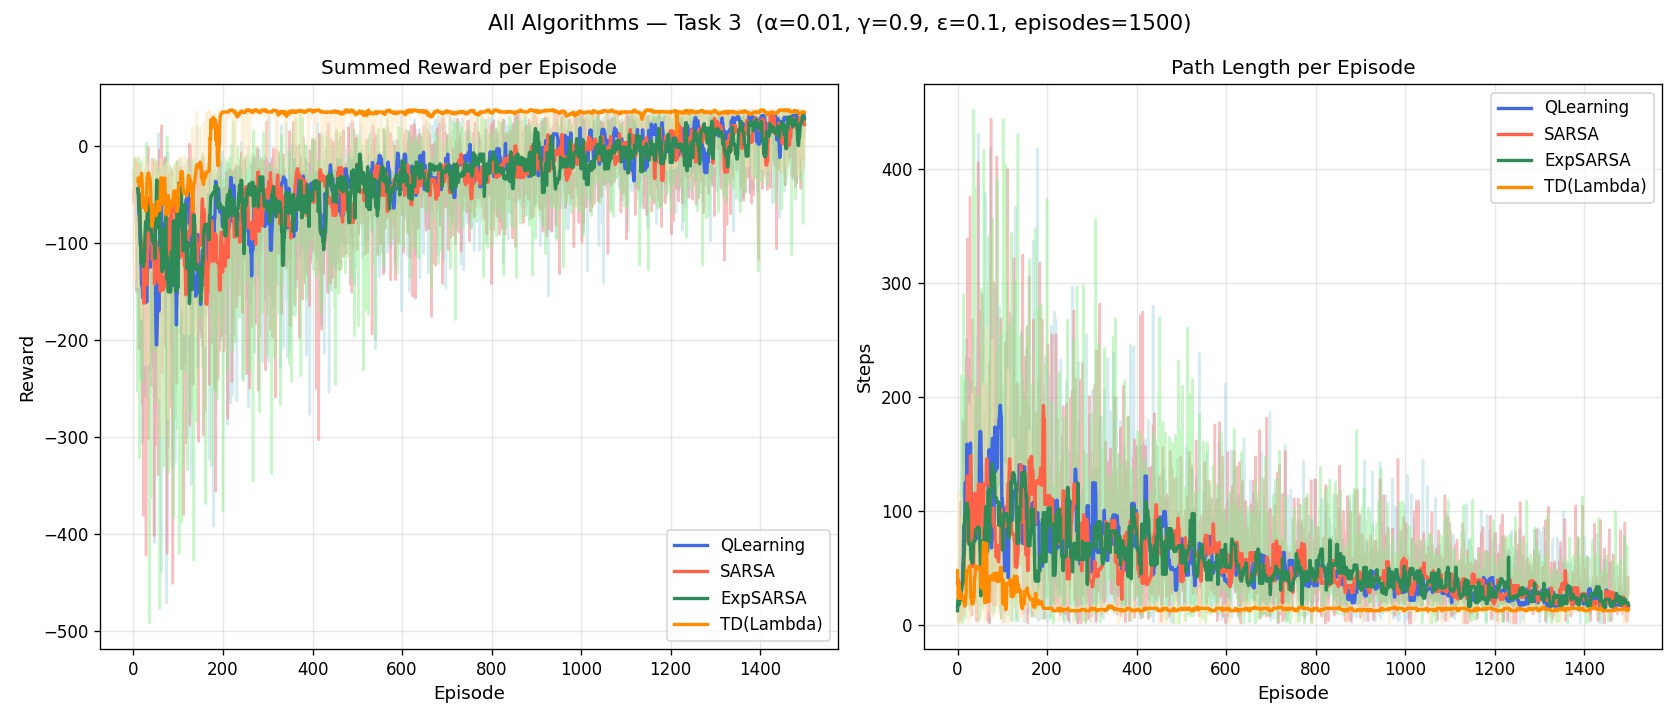
\includegraphics[width=\linewidth]{joint_task3_all_algorithms.png}
    \caption{Task 3 -- all algorithms}
  \end{subfigure}
  \hfill
  \begin{subfigure}{0.48\textwidth}
    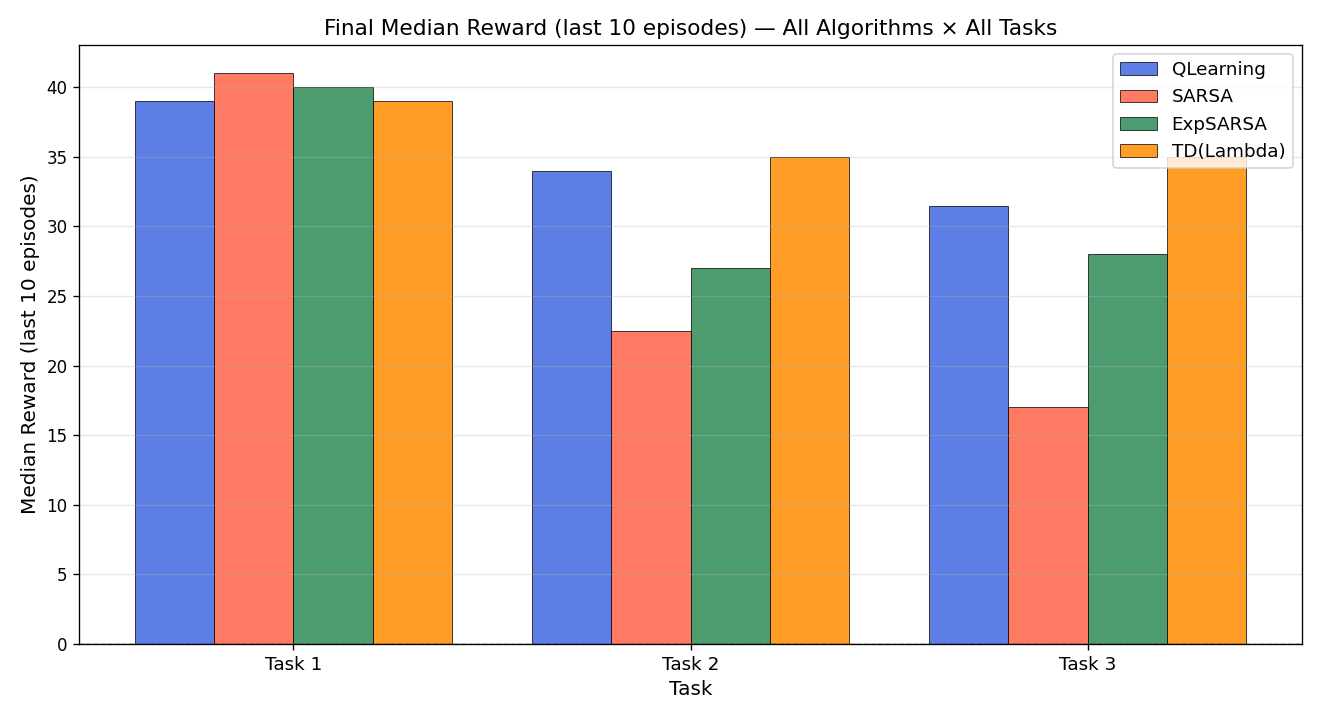
\includegraphics[width=\linewidth]{summary_final_median_all_tasks.png}
    \caption{Final median reward summary}
  \end{subfigure}
  \caption{Reward convergence curves and summary bar chart. Solid lines show the
  rolling median (window=10); faded lines show raw per-episode reward.}
\end{figure}

\begin{figure}[h!]
  \centering
  \begin{subfigure}{0.48\textwidth}
    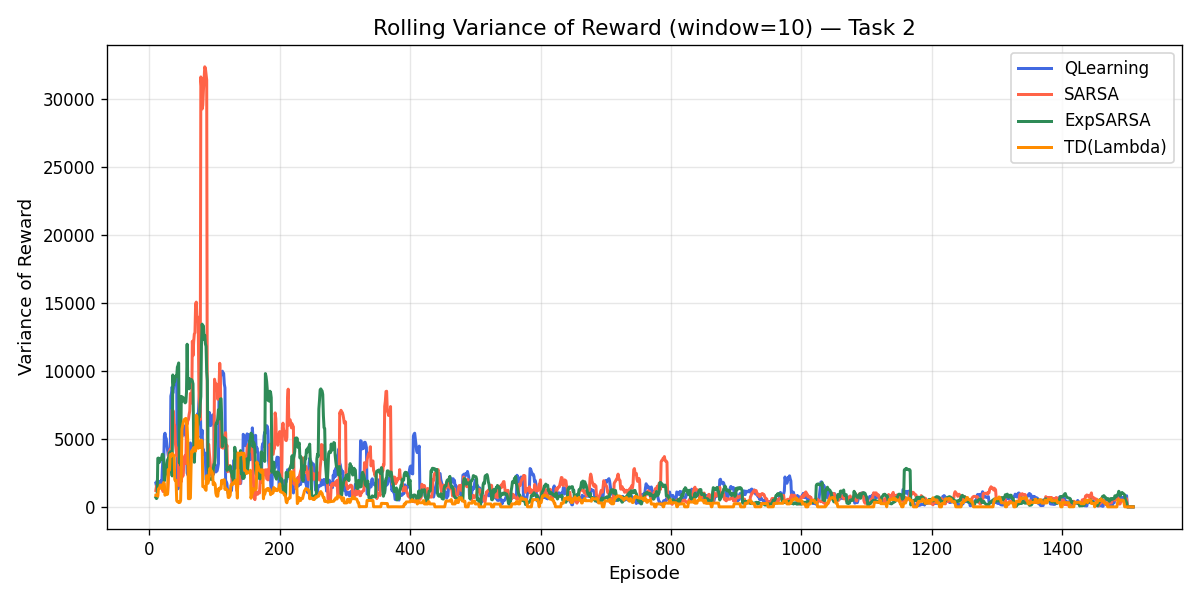
\includegraphics[width=\linewidth]{variance_task2.png}
    \caption{Rolling variance -- Task 2}
  \end{subfigure}
  \hfill
  \begin{subfigure}{0.48\textwidth}
    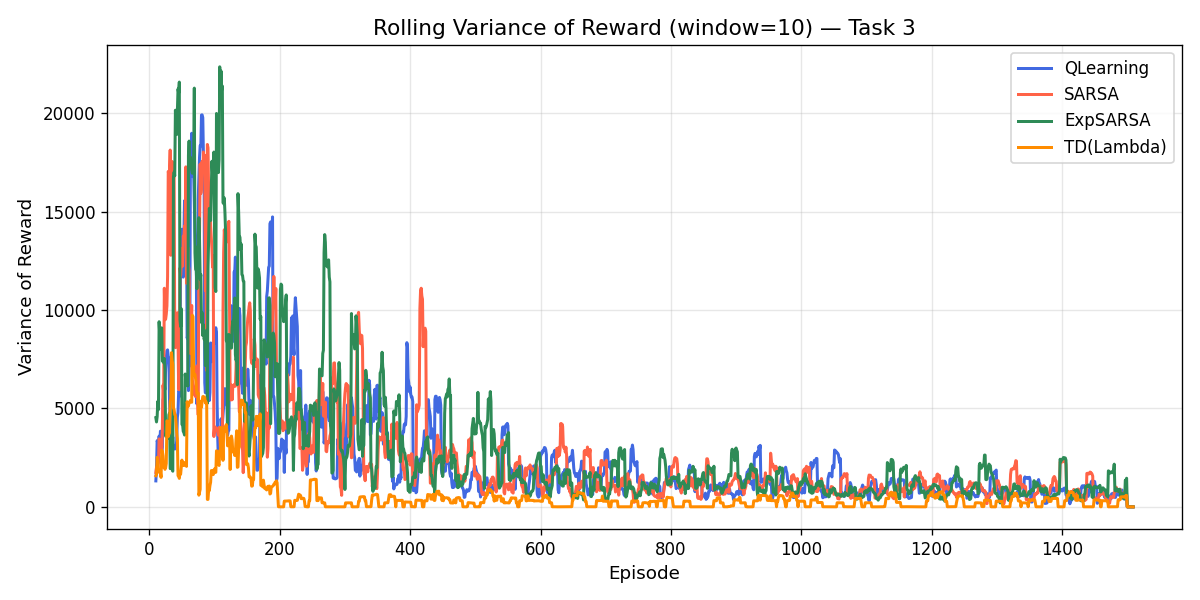
\includegraphics[width=\linewidth]{variance_task3.png}
    \caption{Rolling variance -- Task 3}
  \end{subfigure}
  \caption{Variance of reward over a rolling window of 10 episodes on the complex maps.
  Lower variance indicates more consistent policy execution.}
\end{figure}

% ─────────────────────────────────────────────────────────────────────────────
\section{Results Analysis}

\subsection{Task 1 (simple map -- 8 walls, 3 pits)}

All four algorithms converge to near-optimal policies. The maximum achievable reward
is 41 (9 steps, no pits), which every algorithm achieves in its best episode.

Q-Learning and SARSA reach Med-10~$=$~41 with low variance ($<$2), indicating
reliable policy execution by episode 1500. Expected SARSA also achieves Med-10~$=$~41
but with slightly higher variance (6.56), likely because its expected-value target
produces smaller TD errors early in training, slowing the rate at which Q-values
for good actions separate from those for poor actions. TD($\lambda$) achieves
Med-10~$=$~40 with the highest variance (7.40) on this task, as the trace broadcasts
can occasionally reinforce suboptimal paths when the agent re-explores a previously
visited corridor.

\subsection{Task 2 (pit-heavy map -- 10 pits)}

This is where the algorithms diverge significantly.
TD($\lambda$) achieves \textbf{Med-10~$=$~36, Var-10~$=$~36.4}, the best of all
algorithms by a large margin. The eligibility trace mechanism is directly responsible:
the first time the agent successfully navigates a pit corridor, every step of that
trajectory is immediately reinforced. One-step methods must propagate this corridor
value backwards over many future episodes.

Q-Learning drops sharply to Med-10~$=$~20 with extremely high variance (590.76).
This is the ``reckless off-policy'' effect: the greedy max target assumes the agent
will always execute the greedy action in the future, causing it to plan routes
immediately adjacent to pits. When $\varepsilon$-exploration fires near a pit, the
agent falls in, causing dramatic reward swings.

SARSA (Med-10~$=$~28) and Expected SARSA (Med-10~$=$~30) perform better than Q-Learning
due to their on-policy updates encoding caution near pits. Unexpectedly, Expected SARSA
outperforms SARSA on Task 2 despite SARSA being more commonly cited as ``safer''.

\subsection{Task 3 (diagonal wall barrier -- 6 pits)}

TD($\lambda$) achieves its most dramatic advantage: \textbf{Med-10~$=$~36.5,
Var-10~$=$~1.89}, nearly perfect convergence on the hardest task.

Task 3 features a diagonal wall forcing navigation through a narrow corridor
(columns~3--4, rows~2--4). This is precisely the scenario where eligibility traces
provide maximum value: the corridor must be traversed early in the episode, and
credit must propagate backwards through several steps to reinforce it. One-step
methods require many more episodes to propagate the corridor's value to its entry.

Expected SARSA collapses on Task 3: Med-10~$=$~18, Var-10~$=$~516.69. The expected
value's averaging over the action distribution reduces the magnitude of Q-value
updates at the corridor entry: the uniform component
$\frac{\varepsilon}{|A|}\sum_{a'}Q(s',a')$ includes low-value actions that lead
into walls and pits, pulling the TD target $\delta$ downward and slowing the rate
at which the corridor entry's Q-value separates from surrounding states.
This is the same averaging property that reduces variance on simple maps,
but here it delays convergence precisely where a large, decisive update is needed.

SARSA shows high variance (415.49). The diagonal wall creates two distinct solution
regions; $\varepsilon$-exploration intermittently sends the agent between them even
after partial convergence.

\subsection{Computation Time}

All 1500-episode runs complete in under 60 seconds. The critical optimization
is the dictionary-based Q-table: $O(1)$ state lookup vs.\ $O(n^2)$ DataFrame
appends. The second optimization is the \texttt{maze\_env.py} sleep removal
(see Section 3). TD($\lambda$) has the highest per-step cost at
$O(|S_{\text{visited}}| \times 4)$, but with a maximum of 86 reachable states
this is negligible.

% ─────────────────────────────────────────────────────────────────────────────
\section{Qualitative Observations}

\textbf{Q-Learning} plans aggressively, hugging pit boundaries for shortest paths.
On simple maps this is effective; on pit-dense maps, $\varepsilon$-exploration
causes frequent falls, producing high variance. The off-policy max target instills
zero ``fear'' of future exploration errors.

\textbf{SARSA} is more conservative. Its on-policy updates implicitly penalize
routes near pits because the expected value of being near a pit includes the
probability of $\varepsilon$-exploration into it. This produces cautious, longer
routes but avoids catastrophic falls. Task 3's topology defeats this conservatism,
as the only path through the diagonal wall forces multiple near-pit states.

\textbf{Expected SARSA} is the most variance-stable on simple maps (lowest Var-10 on
Task 1 across multiple runs). The analytical expectation removes noise from the update
target. However, this same stability causes delayed learning on complex maps, as the
average over all actions is less reactive to the widening gap between good-action
and poor-action Q-values than a single greedy or sampled estimate.

\textbf{TD($\lambda$)} learns fastest and converges most reliably on complex maps.
The trajectory plot for Task 2 (Figure~\ref{fig:traj}) visually confirms: early
episodes (red) show random walks; late episodes (green) show tight, consistent paths
through the corridor. The transition from random to directed behavior occurs notably
earlier than in the single-step methods.

\begin{figure}[h!]
  \centering
  \begin{subfigure}{0.48\textwidth}
    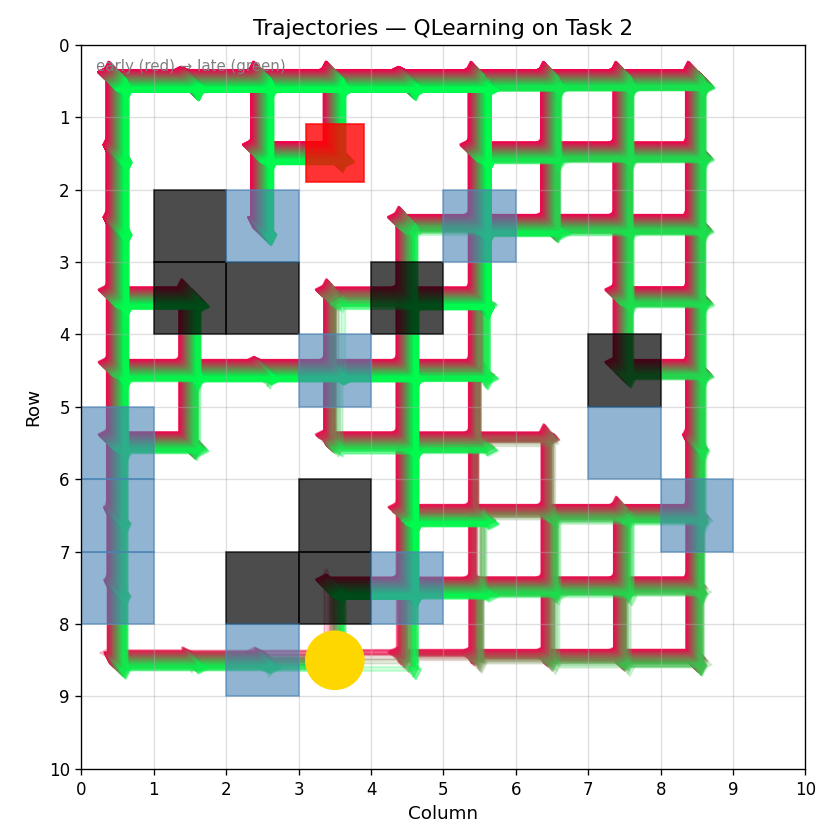
\includegraphics[width=\linewidth]{qlearning_task2_trajectory.png}
    \caption{Q-Learning trajectories -- Task 2}
  \end{subfigure}
  \hfill
  \begin{subfigure}{0.48\textwidth}
    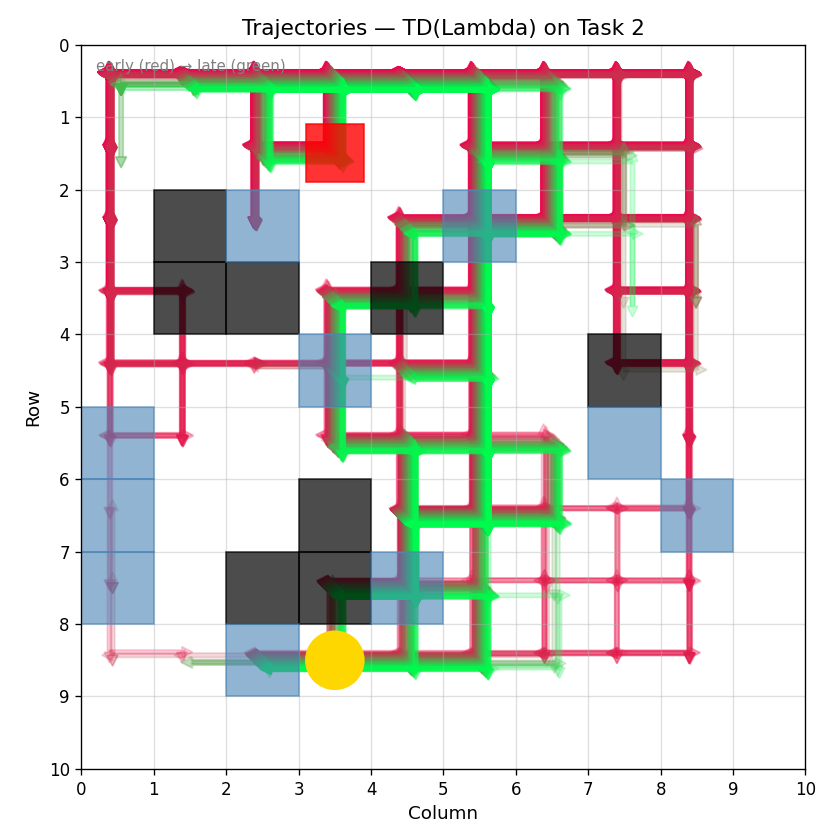
\includegraphics[width=\linewidth]{tdlambda_task2_trajectory.png}
    \caption{TD($\lambda$) trajectories -- Task 2}
  \end{subfigure}

  \vspace{0.5em}
  \begin{subfigure}{0.48\textwidth}
    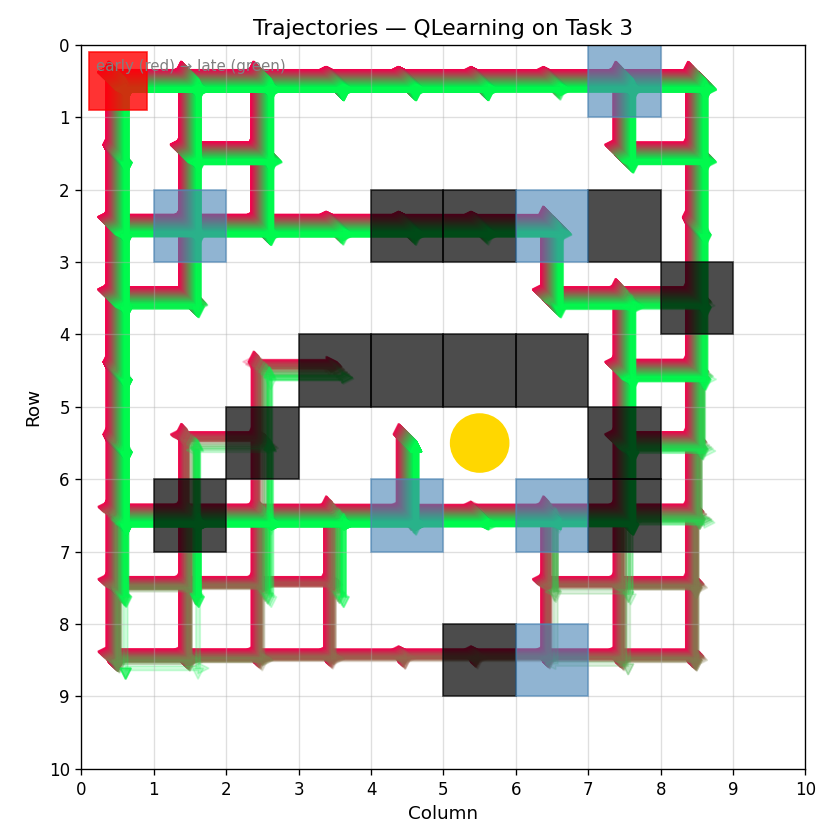
\includegraphics[width=\linewidth]{qlearning_task3_trajectory.png}
    \caption{Q-Learning trajectories -- Task 3}
  \end{subfigure}
  \hfill
  \begin{subfigure}{0.48\textwidth}
    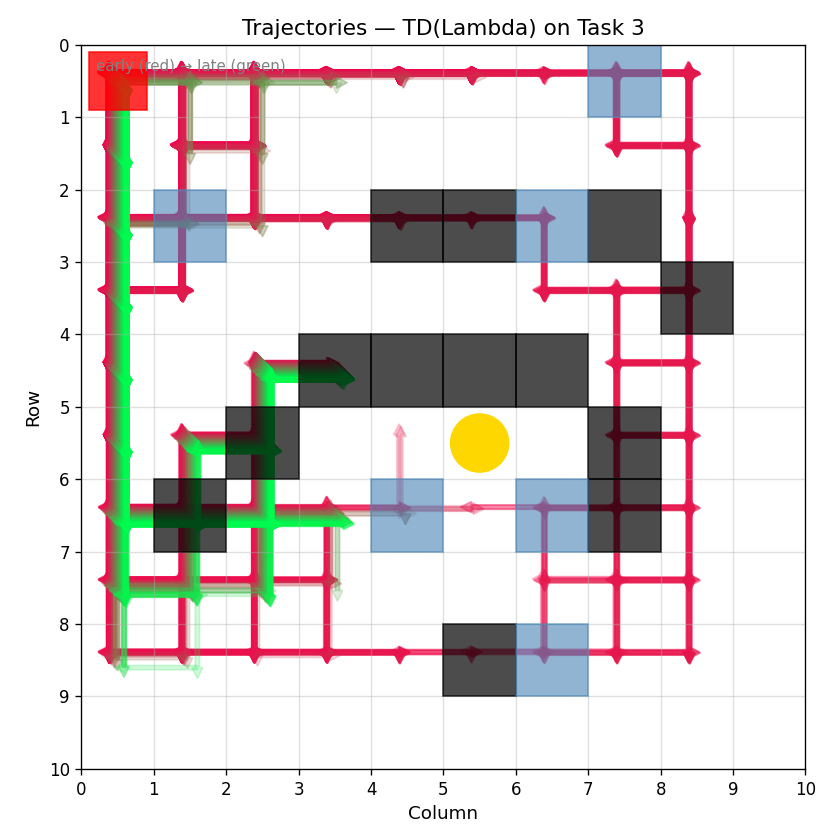
\includegraphics[width=\linewidth]{tdlambda_task3_trajectory.png}
    \caption{TD($\lambda$) trajectories -- Task 3}
  \end{subfigure}

  \caption{Trajectory heatmaps for Tasks 2 and 3. Red = early episodes, green = late
  episodes. Black = walls, blue = pits, gold = goal, red square = start.}
  \label{fig:traj}
\end{figure}

% ─────────────────────────────────────────────────────────────────────────────
\section{Comparison to Search Algorithms (Tasks 2 and 3)}

Tasks~2 and 3 use identical maps to \texttt{task324} and \texttt{task325} from
Assignment~1, enabling direct comparison between RL agents and classical search.

\begin{table}[h!]
\centering
\caption{Search algorithm results on task324 (Task 2) and task325 (Task 3)}
\begin{tabular}{llrrl}
\toprule
\textbf{Map} & \textbf{Algorithm} & \textbf{Path Cost} & \textbf{States Explored} & \textbf{Optimal?} \\
\midrule
task324 (Task 2) & BFS           & 16.8 & 102 & No  \\
task324 (Task 2) & UCS           &  9.2 & 109 & Yes \\
task324 (Task 2) & A* (Euclidean)&  9.2 &  56 & Yes \\
task324 (Task 2) & A* (Manhattan)&  9.2 &  50 & Yes \\
task324 (Task 2) & Greedy BFS    & 25.8 &  25 & No  \\
\midrule
task325 (Task 3) & BFS           &  8.2 &  57 & Yes \\
task325 (Task 3) & UCS           &  8.2 &  57 & Yes \\
task325 (Task 3) & A* (Euclidean)&  8.2 &  33 & Yes \\
task325 (Task 3) & Greedy BFS    & 11.1 &  27 & No  \\
\bottomrule
\end{tabular}
\end{table}



The RL reward model encodes: max reward $= 50 - \text{steps}$ (for a pit-free path).
The best RL rewards (Table~\ref{tab:results}) imply:
\begin{itemize}[noitemsep]
  \item Task 2 best RL path: $50 - 38 = 12$ steps \quad vs.\ A* optimal: $\approx 9$ steps
  \item Task 3 best RL path: $50 - 37 = 13$ steps \quad vs.\ A* optimal: $\approx 8$ steps
\end{itemize}

RL finds paths approximately 30--60\% longer than the search-optimal solution.

\subsection{Key Differences}

\begin{description}
  \item[Optimality guarantee.] A*/UCS guarantee the optimal path given an admissible
    heuristic. RL provides no such guarantee and converges to near-optimal but not
    provably optimal policies. Both Euclidean and Manhattan distance are admissible
    for this grid, so A* finds the true optimum.

  \item[Sample efficiency.] A* explores 33--56 unique states to find the solution.
    RL agents visit states millions of times over 1500 episodes. Search is orders of
    magnitude more efficient for known, static environments.

  \item[Prior knowledge requirement.] A* and UCS require a complete model: the
    transition function, all states, and step costs. RL requires only reward signals
    from direct interaction, no map is needed.

  \item[Policy coverage.] Search returns a single path from the start state. RL
    produces a complete policy $\pi(s)$ over every state in the maze. If the agent is
    displaced mid-episode (stochastic transition, noisy actuation), the RL policy
    handles it; a search path cannot.

  \item[Stochastic environments.] Both A* and UCS assume deterministic transitions.
    RL handles stochastic dynamics naturally. For this static, deterministic maze the
    distinction does not apply, which is precisely why search outperforms RL on
    raw path quality.
\end{description}

\subsection{Observation: BFS on task325}

On task325 (= Task~3), BFS finds the same cost as UCS and A* (8.2). This means the
optimal path contains no pits, as BFS's cost-agnostic search happens to find the
optimal-cost path because the shortest-hop path is also the cheapest. This is a
non-obvious property of the specific map geometry and is consistent with the RL
agents' best episodes also being pit-free (reward $= 37 = 50 - 13$, no $-10$
pit penalties).

% ─────────────────────────────────────────────────────────────────────────────
\section{Conclusion}

TD($\lambda$) is the most effective algorithm on complex maps due to its multi-step
credit assignment via eligibility traces. It achieves the highest median reward on
Tasks~2 and~3 and the lowest variance on Task~3, confirming that backward credit
propagation is particularly valuable when the maze contains structural bottlenecks
(corridors, diagonal walls).

Q-Learning performs well on simple maps but degrades under dense pit configurations
due to its off-policy recklessness. SARSA offers a stable, cautious baseline.
Expected SARSA provides the lowest variance on simple maps but fails to converge
reliably on Task~3 because its averaged TD target slows the rate at which Q-values
separate near critical narrow passages.

Compared to classical search (A*, UCS), RL requires substantially more computation
and finds suboptimal paths (30--60\% longer than optimal). However, RL operates
without a world model and produces a complete policy over all states, properties
essential in real-world environments where a precomputed map is unavailable.

\section{GitLab Repo}

\url{https://git.uwaterloo.ca/sradebam/asg2-w26}

\end{document}
